\chapter{Near the Horizon of a Schwarzschild Black Hole}

Before beginning the promised journey into a large black hole, Leonard Susskind deliberately returns to the accelerated frame. That is the right place to begin, because the near-horizon region of a Schwarzschild black hole turns out to look like flat spacetime written in accelerated coordinates. In these notes we follow that progression closely: first the hyperbolic geometry of accelerated observers, then the observational story of Alice and Bob, then the Schwarzschild metric and its suspicious radii, then the near-horizon approximation, and finally the interior singularity and the vacuum field equations outside matter. The chapter follows Leonard Susskind's lecture, with the archival lecture record preserved by LazyingArt LLC and Video2Book.

\section{Accelerated Observers and Hyperbolic Coordinates}

Let us recall the accelerated frame in flat spacetime. The key point is that this is not only a coordinate change. We first rewrite Minkowski space in a new set of coordinates, and then we imagine a family of observers who sit at fixed values of the new spatial coordinate. Those fixed-coordinate observers are accelerated observers.

In the freely falling Minkowski coordinates \((X,T)\), the hyperbolic coordinates are defined by
\begin{equation}
X = r\cosh\omega,
\qquad
T = r\sinh\omega.
\end{equation}
The coordinate \(r\) labels the hyperbolic worldline, while \(\omega\) is the hyperbolic angle. It plays the role of time in the accelerated frame, but it is not the proper time of every observer. Indeed, the closer a trajectory lies to the light cone, the more sharply it bends, and the larger the proper acceleration required to hold the observer there.

From the coordinate map we immediately obtain
\begin{equation}
X^2 - T^2 = r^2,
\qquad
\frac{T}{X} = \tanh\omega.
\end{equation}
Thus the curves of constant \(r\) are hyperbolae, while the curves of constant \(\omega\) are straight rays through the origin.

Now let us write the metric. In ordinary Minkowski coordinates,
\begin{equation}
d\tau^2 = dT^2 - dX^2 - dy^2 - dz^2.
\end{equation}
Substituting the hyperbolic coordinates gives
\begin{align}
d\tau^2
&= r^2\,d\omega^2 - dr^2 - dy^2 - dz^2.
\end{align}
Along a fixed-\(r\) trajectory, with \(dr=dy=dz=0\), this reduces to
\begin{equation}
d\tau = r\,d\omega.
\end{equation}
This is one of the important reminders from the lecture: clocks that measure proper time do not all tick off \(\omega\) at the same rate. If one insists on using \(\omega\) as a common time coordinate for the accelerated frame, then the clocks at different \(r\) must be adjusted differently.

\begin{figure}[htbp]
\centering

\includegraphics[width=0.78\textwidth]{lecture_12_figure_02.png}

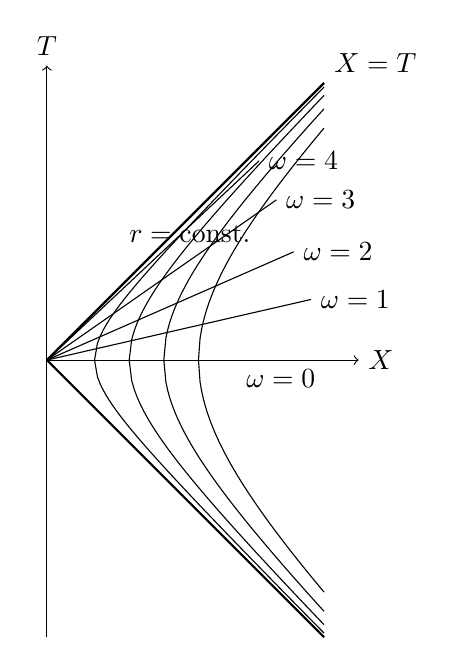
\begin{tikzpicture}[scale=1.1]
\draw[->] (0,-3.2) -- (0,3.4) node[above] {$T$};
\draw[->] (0,0) -- (3.6,0) node[right] {$X$};
\draw[thick] (0,0) -- (3.2,3.2) node[above right] {$X=T$};
\draw[thick] (0,0) -- (3.2,-3.2);

\draw[domain=0.55:3.2,samples=80] plot (\x,{sqrt(\x*\x-0.55*0.55)});
\draw[domain=0.55:3.2,samples=80] plot (\x,{-sqrt(\x*\x-0.55*0.55)});
\draw[domain=0.95:3.2,samples=80] plot (\x,{sqrt(\x*\x-0.95*0.95)});
\draw[domain=0.95:3.2,samples=80] plot (\x,{-sqrt(\x*\x-0.95*0.95)});
\draw[domain=1.35:3.2,samples=80] plot (\x,{sqrt(\x*\x-1.35*1.35)});
\draw[domain=1.35:3.2,samples=80] plot (\x,{-sqrt(\x*\x-1.35*1.35)});
\draw[domain=1.75:3.2,samples=80] plot (\x,{sqrt(\x*\x-1.75*1.75)});
\draw[domain=1.75:3.2,samples=80] plot (\x,{-sqrt(\x*\x-1.75*1.75)});

\draw (0,0) -- (3.2,0);
\draw (0,0) -- (3.05,0.7);
\draw (0,0) -- (2.85,1.25);
\draw (0,0) -- (2.65,1.85);
\draw (0,0) -- (2.45,2.3);

\node[below] at (2.7,0) {$\omega=0$};
\node[right] at (3.05,0.7) {$\omega=1$};
\node[right] at (2.85,1.25) {$\omega=2$};
\node[right] at (2.65,1.85) {$\omega=3$};
\node[right] at (2.45,2.3) {$\omega=4$};
\node at (1.65,1.45) {$r=\mathrm{const.}$};
\end{tikzpicture}
\caption{The accelerated frame: constant-\(r\) hyperbolae, constant-\(\omega\) rays, and the limiting lightlike line \(X=T\). The board frame is kept as documentary evidence for the original diagram and labeling.}
\end{figure}

The line \(X=T\) is the limiting horizon of this accelerated coordinate system. The ray \(\omega=0\) is the horizontal slice \(T=0\), and as \(\omega\to\infty\), the rays pile up against the lightlike boundary \(X=T\). Nothing in the accelerated description reaches that boundary at finite \(\omega\).

\section{Alice, Bob, and the Horizon as a Visual Limit}

Once the geometry is on the board, the lecture immediately turns from coordinates to observation. Susskind's point is that ``seeing'' means receiving light, and therefore seeing always involves looking backward along null lines.

Suppose Alice lets go and falls through the horizon, while Bob remains supported outside, riding one of the accelerated trajectories. Bob can only see Alice by looking backward along lightlike directions from his own worldline. Each time he looks, the light that reaches him comes from a point on Alice's trajectory closer to the horizon than the last one. In Bob's description, Alice approaches the horizon asymptotically. She never seems to cross it in any finite value of the accelerated time.

\begin{figure}[htbp]
\centering

\includegraphics[width=0.82\textwidth]{lecture_12_figure_04.png}

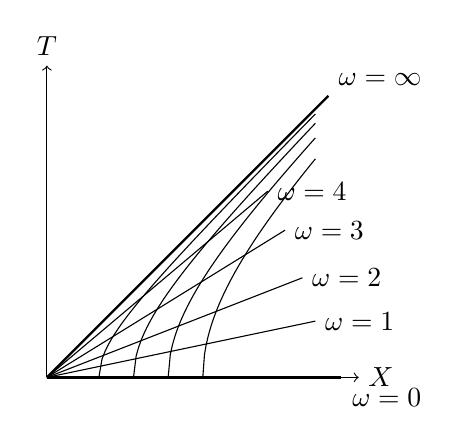
\begin{tikzpicture}[scale=1.1]
\draw[->] (0,0) -- (3.6,0) node[right] {$X$};
\draw[->] (0,0) -- (0,3.6) node[above] {$T$};
\draw[thick] (0,0) -- (3.25,3.25) node[above right] {$\omega=\infty$};
\draw[very thick] (0,0) -- (3.4,0) node[below right] {$\omega=0$};
\draw (0,0) -- (3.1,0.65);
\draw (0,0) -- (2.95,1.15);
\draw (0,0) -- (2.75,1.7);
\draw (0,0) -- (2.55,2.15);

\draw[domain=0.6:3.1,samples=70] plot (\x,{sqrt(\x*\x-0.6*0.6)});
\draw[domain=1.0:3.1,samples=70] plot (\x,{sqrt(\x*\x-1.0*1.0)});
\draw[domain=1.4:3.1,samples=70] plot (\x,{sqrt(\x*\x-1.4*1.4)});
\draw[domain=1.8:3.1,samples=70] plot (\x,{sqrt(\x*\x-1.8*1.8)});

\node[right] at (3.1,0.65) {$\omega=1$};
\node[right] at (2.95,1.15) {$\omega=2$};
\node[right] at (2.75,1.7) {$\omega=3$};
\node[right] at (2.55,2.15) {$\omega=4$};
\end{tikzpicture}
\caption{The accelerated time slices pile up against the horizon. This is the visual content of the statement that the horizon is reached only at \(\omega=\infty\) in the accelerated description.}
\end{figure}

Alice, however, does not report anything dramatic when she crosses the horizon. She simply falls through. If she looks back, she sees Bob receding away on an accelerated trajectory. She can see his motions slow, but she does not see a special local event at the horizon.

\subsection{Question \& Answer}

\paragraph{Question.} Why does Bob see asymptotic freezing while Alice notices no special event at the horizon?

\paragraph{Answer.} The asymmetry comes from the way signals reach the two observers. Bob remains supported outside and uses the accelerated time coordinate. For him the horizon sits at \(\omega=\infty\), so light sent by Alice reaches him from points ever closer to that limiting line. His past light cone samples Alice more and more slowly, and her clock appears to slow down.

Alice does not use that accelerated slicing. She is in free fall, and the local geometry near the horizon is smooth. In her own proper time the crossing occurs after a finite interval. When she looks back she sees Bob moving away, and so she also sees some slowing due to recession, but not because the horizon is itself a place of local catastrophe. The freezing is therefore a statement about Bob's coordinates and Bob's received signals, not a statement that the horizon is a physical wall.

\section{The Schwarzschild Metric and Its Suspicious Radii}

Having restored the accelerated picture, Susskind now writes the Schwarzschild metric and announces the real task of the day: to connect that metric to the Rindler-like geometry we have just recalled.

Setting \(c=1\), the Schwarzschild line element is
\begin{equation}
d\tau^2
=
\left(1-\frac{2MG}{r}\right)dt^2
-
\frac{dr^2}{1-\frac{2MG}{r}}
-
r^2\,d\Omega^2,
\qquad
d\Omega^2 = d\theta^2 + \sin^2\theta\,d\phi^2.
\end{equation}
This is the exterior metric of a spherically symmetric gravitating body. In particular, it describes not only an ideal Schwarzschild black hole, but also the gravitational field outside the surface of the Earth.

\begin{figure}[htbp]
\centering

\includegraphics[width=0.82\textwidth]{lecture_12_figure_03.png}
\caption{The Schwarzschild line element on the board. The left edge is slightly cropped, so the displayed equation above gives the clean standard form.}
\end{figure}

There are two suspicious radii:
\begin{equation}
r=2MG,
\qquad
r=0.
\end{equation}
At \(r=2MG\), the coefficient of \(dt^2\) goes to zero and the coefficient of \(dr^2\) blows up. That looks ominous. But we have already seen a warning example in flat spacetime: a coefficient can vanish while its partner diverges, simply because the coordinates are badly chosen.

To make that warning explicit, Susskind briefly returns to the accelerated metric and renames the old radial variable \(\rho\), reserving \(r\) from now on for the Schwarzschild areal radius. If we then define
\begin{equation}
R = \rho^2,
\end{equation}
the flat accelerated metric becomes
\begin{equation}
d\tau^2
=
R\,d\omega^2
-
\frac{dR^2}{4R}
-
dy^2
-
dz^2.
\end{equation}
At \(R=0\), one coefficient vanishes and the other diverges. But spacetime is still flat. That is the whole point of the toy model: a singular-looking metric coefficient is not yet a physical singularity.

The continuation also explains the sign flip. Since
\begin{equation}
X^2-T^2=\rho^2=R,
\end{equation}
the region \(R<0\) is simply the region where
\begin{equation}
T^2-X^2=-R.
\end{equation}
Nothing mystical has happened. The coordinates have merely been pushed through the light cone in a way that changes which coordinate is timelike and which is spacelike.

By contrast, \(r=0\) in the Schwarzschild geometry is not just a coordinate nuisance. There the lecture insists on a stronger statement: tidal forces become infinite, and one truly encounters a curvature singularity.

\section{Near the Horizon: From Schwarzschild to Rindler}

Now comes the main derivation. We do not want the exact global Schwarzschild geometry; we want the geometry in a very small neighborhood near one point of the horizon. That is enough to decide whether the horizon itself is singular.

Let us first rewrite the metric:
\begin{equation}
d\tau^2
=
\frac{r-2MG}{r}\,dt^2
-
\frac{r}{r-2MG}\,dr^2
-
r^2\,d\Omega^2.
\end{equation}
Near the horizon, \(r\) is very close to \(2MG\). The important small quantity is \(r-2MG\). Therefore we keep \(r-2MG\) explicit, but in the slowly varying denominators we replace \(r\) by \(2MG\). This gives the near-horizon approximation
\begin{equation}
d\tau^2
\approx
\frac{r-2MG}{2MG}\,dt^2
-
\frac{2MG}{r-2MG}\,dr^2
-
(2MG)^2\,d\Omega^2.
\end{equation}

Next, we zoom in on one point of the horizon sphere. A sufficiently small patch of a sphere looks flat, so the angular part may be replaced by the metric of a tangent plane:
\begin{equation}
(2MG)^2\,d\Omega^2 \approx dy^2 + dz^2.
\end{equation}
Thus the local metric becomes
\begin{equation}
d\tau^2
\approx
\frac{r-2MG}{2MG}\,dt^2
-
\frac{2MG}{r-2MG}\,dr^2
-
dy^2
-
dz^2.
\end{equation}

Now comes the decisive coordinate choice. We define \(\rho\) to be the proper spatial distance from the horizon. If we move outward at fixed \(t\), \(y\), and \(z\), then the proper distance element is determined entirely by the radial term:
\begin{equation}
d\rho^2
=
\frac{2MG}{r-2MG}\,dr^2.
\end{equation}
This is not guessed; it is chosen precisely so that the radial part of the metric becomes \(-d\rho^2\).

Integrating from the horizon \(r=2MG\) to an outside point \(r\), we find
\begin{align}
\rho
&=
\int_{2MG}^{r}
\sqrt{\frac{2MG}{r'-2MG}}\,dr' \\
&=
2\sqrt{2MG}\,\sqrt{r-2MG} \\
&=
\sqrt{8MG}\,\sqrt{r-2MG}.
\end{align}
Therefore
\begin{equation}
r-2MG = \frac{\rho^2}{8MG}.
\end{equation}
Substituting this into the time term gives
\begin{equation}
\frac{r-2MG}{2MG}\,dt^2
=
\frac{\rho^2}{16M^2G^2}\,dt^2.
\end{equation}
So the metric reads
\begin{equation}
d\tau^2
=
\frac{\rho^2}{16M^2G^2}\,dt^2
-
d\rho^2
-
dy^2
-
dz^2.
\end{equation}

The last step is a simple rescaling of time:
\begin{equation}
\omega = \frac{t}{4MG},
\qquad
d\omega = \frac{dt}{4MG}.
\end{equation}
Then
\begin{equation}
d\tau^2
=
\rho^2\,d\omega^2
-
d\rho^2
-
dy^2
-
dz^2.
\end{equation}
This is exactly the accelerated-frame metric we started with. Near one point on the horizon, the Schwarzschild metric becomes the Rindler metric.

\begin{figure}[htbp]
\centering

\includegraphics[width=0.72\textwidth]{lecture_12_figure_05.png}
\caption{The near-horizon metric block and the time rescaling \(\omega=t/(4MG)\) on the board. The image is blurred in places, so the typeset equations above carry the mathematical burden.}
\end{figure}

That is the payoff of the whole calculation. The horizon is not a curvature singularity. Very near the horizon, and very near one chosen point on it, the geometry is simply flat spacetime in accelerated coordinates.

\section{What the Horizon Does and Does Not Mean}

The calculation tells us two things at once. First, the horizon is locally harmless: a freely falling observer can cross it without encountering any singular local geometry. Second, the horizon remains special as a causal boundary for observers who do not fall through.

Close to the horizon, the Schwarzschild time behaves like a hyperbolic angle:
\begin{equation}
\omega = \frac{t}{4MG}.
\end{equation}
Far from the horizon, by contrast, \(2MG/r\) is negligible, and the Schwarzschild metric approaches ordinary flat spacetime in ordinary coordinates. The lecture emphasizes this contrast repeatedly. Near the horizon one naturally thinks in Rindler-like coordinates; far away one naturally thinks in standard \(t\) and \(r\).

For an observer who stays supported outside, nothing is ever seen to cross the horizon. An infalling object can send light signals outward, but the received intervals stretch more and more. The signal is redshifted through optical light, infrared, microwave, radio, and beyond. In Susskind's wave-train picture, a finite-frequency source produces only finitely many recognizable crests before the signal is effectively lost into infinite delay.

This is why Bob says that Alice freezes, reddens, and disappears into the horizon. The horizon is not singular, but it is the limit of no return for the outside description. From that same outside point of view, infalling matter piles up closer and closer to the horizon, and the black hole grows because the horizon grows to include the infalling energy.

There is another instructive point here. One might ask whether an object could skirt along the horizon, moving only in the transverse directions \(y\) or \(z\). The answer is no. If we keep \(r\) fixed and set \(dr=0\), then near the horizon
\begin{equation}
d\tau^2
\approx
\frac{r-2MG}{2MG}\,dt^2
-
dy^2
-
dz^2.
\end{equation}
As \(r\to 2MG\), the coefficient of \(dt^2\) becomes arbitrarily small. A transverse displacement of fixed size then overwhelms the timelike part and makes the trajectory spacelike. So no timelike observer can skim along the horizon. That would require faster-than-light motion.

\section{Inside the Horizon and the Nature of the Singularity}

Up to now the lecture has been mainly about what is \emph{not} singular. Now it turns to what really is singular. The singularity is at \(r=0\), and the key question is: where does that sit in the causal picture?

Inside the horizon we have
\begin{equation}
r<2MG
\qquad\Longrightarrow\qquad
1-\frac{2MG}{r}<0.
\end{equation}
Therefore the coefficient of \(dt^2\) becomes negative and the coefficient of \(dr^2\) becomes positive. But here again Susskind is careful: this sign exchange is not itself a physical statement that time has literally become space. It is a statement about the coordinates. The earlier toy model with \(R=\rho^2\) already showed how such a sign change can arise when coordinates are continued through a horizon.

What \emph{is} physically important is that fixed Schwarzschild \(r\) no longer describes the worldline of a supported observer once we are inside the horizon. Outside the hole, fixed \(r\) is timelike. Inside the hole, fixed \(r\) is spacelike. In Susskind's phrase, fixed \(r\) inside is ``some time, not some place.''

\begin{figure}[htbp]
\centering
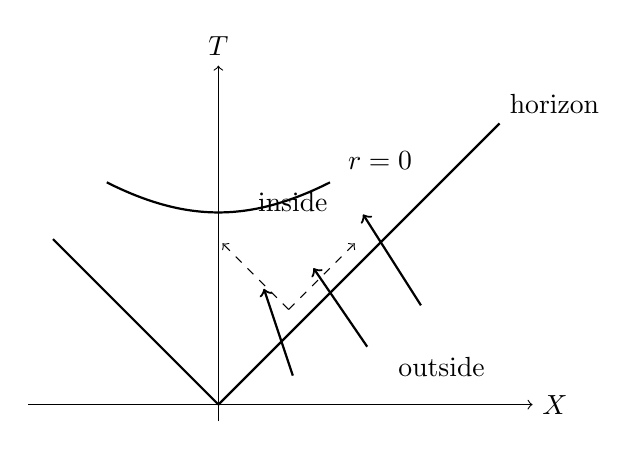
\begin{tikzpicture}[scale=1.05]
\draw[->] (-2.3,0) -- (3.8,0) node[right] {$X$};
\draw[->] (0,-0.2) -- (0,4.1) node[above] {$T$};

\draw[thick] (0,0) -- (3.4,3.4) node[above right] {horizon};
\draw[thick] (0,0) -- (-2.0,2.0);

\draw[thick,domain=-1.35:1.35,samples=100] plot (\x,{sqrt(\x*\x+5.4)});
\node[right] at (1.45,2.95) {$r=0$};

\draw[->,thick] (1.8,0.7) -- (1.15,1.65);
\draw[->,thick] (2.45,1.2) -- (1.75,2.3);
\draw[->,thick] (0.9,0.35) -- (0.55,1.4);

\draw[->,dashed] (0.85,1.15) -- (1.65,1.95);
\draw[->,dashed] (0.85,1.15) -- (0.05,1.95);

\node at (2.7,0.45) {outside};
\node at (0.9,2.45) {inside};
\end{tikzpicture}
\caption{A causal redraw of the interior picture. Once inside the horizon, every future-directed timelike or lightlike trajectory ends on the spacelike singularity \(r=0\).}
\end{figure}

The singularity is therefore not best thought of as a point sitting somewhere ahead that one might dodge. It is a spacelike future boundary. Once a trajectory enters the black-hole interior, every future-directed causal path terminates there.

\subsection{Question \& Answer}

\paragraph{Question.} Is the singularity a place one could try to avoid, or is it a future spacelike boundary that one inevitably reaches after crossing the horizon?

\paragraph{Answer.} The lecture's answer is unambiguous. The singularity is not a place in the ordinary sense. If it were merely a point in space, one could imagine missing it. But once the interior geometry is drawn correctly, \(r=0\) is a spacelike surface to the future of every interior event. Inside the horizon, both inward-going and outward-going light rays hit it. Therefore every future-directed timelike or null trajectory reaches the singularity in a finite proper time.

This is the sharp difference between the horizon and the singularity. The horizon is locally innocuous but globally decisive; the singularity is the genuine curvature catastrophe. One crosses the horizon without noticing anything special locally, but after that one is doomed.

The lecture adds an important physical qualification. For a stellar-mass black hole, tidal forces at the horizon are already violent enough to destroy an ordinary human observer. For a sufficiently large black hole, however, the horizon is so large and so nearly flat that one could cross it without appreciable local stress. The real violence then occurs later, at the singularity, not at the horizon.

\section{Vacuum Field Equations, Exterior Solutions, and Why Black Holes Form}

The lecture closes by stepping back and asking where the Schwarzschild metric comes from. Outside the matter distribution there is no local source, so Einstein's equation becomes the vacuum equation
\begin{equation}
R_{\mu\nu}-\frac{1}{2}g_{\mu\nu}R = 0.
\end{equation}
This is the relativistic analog of the Newtonian statement that outside the source the potential satisfies Laplace's equation:
\begin{equation}
\nabla^2\phi = \rho_{\text{mass}},
\qquad
\nabla^2\phi = 0 \quad \text{outside the source.}
\end{equation}

\begin{figure}[htbp]
\centering

\includegraphics[width=0.68\textwidth]{lecture_12_figure_06.png}
\caption{The board comparison between the vacuum Einstein equation and the Newtonian Poisson equation. The lower source term is schematic on the board, so the typeset notation here is normalized.}
\end{figure}

For a spherically symmetric Newtonian potential that vanishes at infinity, the exterior solution is
\begin{equation}
\phi(R) = -\frac{GM}{R}.
\end{equation}
The constant is fixed by the mass contained inside the sphere. This is exactly the analogy Susskind wants at the end: outside the matter, the field is determined by the enclosed mass and by symmetry.

The black-hole case differs sharply from the Newtonian intuition that a point singularity is easy to miss. In Newtonian mechanics, a tiny angular momentum lets matter fly past a point. Einstein at one stage believed something like that would obstruct black-hole formation. But the black-hole singularity is not merely a point in space waiting to be hit. Once matter crosses the horizon, the singularity lies to its future. It is not something the matter can miss.

There is also a clean order-of-magnitude argument for why black holes can form even at low average density. Let a ball of matter have mass \(M\), radius \(R\), and mean density \(\bar\rho\). Then
\begin{equation}
M \sim \bar\rho\,R^3.
\end{equation}
Its Schwarzschild radius is
\begin{equation}
R_{\mathrm S} = 2GM.
\end{equation}
Hence
\begin{equation}
R \sim \left(\frac{M}{\bar\rho}\right)^{1/3}.
\end{equation}
Now compare the two scalings. At fixed mean density, the matter radius grows like \(M^{1/3}\), whereas the Schwarzschild radius grows like \(M\). Therefore, for sufficiently large \(M\),
\begin{equation}
R < R_{\mathrm S}.
\end{equation}
That is precisely the condition for black-hole formation.

Equivalently, at threshold one finds only the scaling
\begin{equation}
\bar\rho_{\mathrm{crit}} \sim \frac{M}{R_{\mathrm S}^3} \propto M^{-2},
\end{equation}
up to numerical factors and the appropriate powers of \(G\) in the chosen units. So the larger the black hole, the smaller the average density needed to form it. That is why black-hole formation is not blocked by the naive Newtonian picture of matter missing a central point.

\section{Summary}

The lecture begins with the accelerated frame because the horizon of a Schwarzschild black hole, when examined locally and near one point, has exactly that geometry. The near-horizon metric is the Rindler metric. This shows that the horizon at \(r=2MG\) is not a curvature singularity. It is nevertheless a limit of no return for observers who remain supported outside.

The real singularity is at \(r=0\). Inside the horizon, fixed Schwarzschild \(r\) becomes spacelike, and the singularity is a spacelike future boundary rather than an ordinary place. Every future-directed causal trajectory inside the hole ends there in finite proper time. Outside matter, the metric is governed by the vacuum Einstein equation, just as the Newtonian potential outside sources satisfies Laplace's equation. And because the Schwarzschild radius grows faster with mass than an ordinary radius at fixed density, sufficiently large masses form black holes even when their average density is small.